\documentclass[11pt,a4paper]{report}
\usepackage[textwidth=37em,vmargin=30mm]{geometry}
\usepackage{calc,xunicode,amsmath,amssymb,paralist,enumitem,tabu,booktabs,datetime2,xeCJK,xeCJKfntef,listings}
\usepackage{tocloft,fancyhdr,tcolorbox,xcolor,graphicx,eso-pic,xltxtra,xelatexemoji}

\newcommand{\envyear}[0]{2025}
\newcommand{\envdatestr}[0]{2025-09-16}
\newcommand{\envfinaldir}[0]{webdb/2025/20250916/final}

\usepackage[hidelinks]{hyperref}
\hypersetup{
    colorlinks=false,
    pdfpagemode=FullScreen,
    pdftitle={Web Digest - \envdatestr}
}

\setlength{\cftbeforechapskip}{10pt}
\renewcommand{\cftchapfont}{\rmfamily\bfseries\large\raggedright}
\setlength{\cftbeforesecskip}{2pt}
\renewcommand{\cftsecfont}{\sffamily\small\raggedright}

\setdefaultleftmargin{2em}{2em}{1em}{1em}{1em}{1em}

\usepackage{xeCJK,xeCJKfntef}
\xeCJKsetup{PunctStyle=plain,RubberPunctSkip=false,CJKglue=\strut\hskip 0pt plus 0.1em minus 0.05em,CJKecglue=\strut\hskip 0.22em plus 0.2em}
\XeTeXlinebreaklocale "zh"
\XeTeXlinebreakskip = 0pt


\setmainfont{Brygada 1918}
\setromanfont{Brygada 1918}
\setsansfont{IBM Plex Sans}
\setmonofont{JetBrains Mono NL}
\setCJKmainfont{Noto Serif CJK SC}
\setCJKromanfont{Noto Serif CJK SC}
\setCJKsansfont{Noto Sans CJK SC}
\setCJKmonofont{Noto Sans CJK SC}

\setlength{\parindent}{0pt}
\setlength{\parskip}{8pt}
\linespread{1.15}

\lstset{
	basicstyle=\ttfamily\footnotesize,
	numbersep=5pt,
	backgroundcolor=\color{black!5},
	showspaces=false,
	showstringspaces=false,
	showtabs=false,
	tabsize=2,
	captionpos=b,
	breaklines=true,
	breakatwhitespace=true,
	breakautoindent=true,
	linewidth=\textwidth
}






\newcommand{\coverpic}[2]{
    % argv: itemurl, authorname
    Cover photo by #2~~(\href{#1}{#1})
}
\newcommand{\makeheader}[0]{
    \begin{titlepage}
        % \newgeometry{hmargin=15mm,tmargin=21mm,bmargin=12mm}
        \begin{center}
            
            \rmfamily\scshape
            \fontspec{BaskervilleF}
            \fontspec{Old Standard}
            \fontsize{59pt}{70pt}\selectfont
            WEB\hfill DIGEST
            
            \vfill
            % \vskip 30pt
            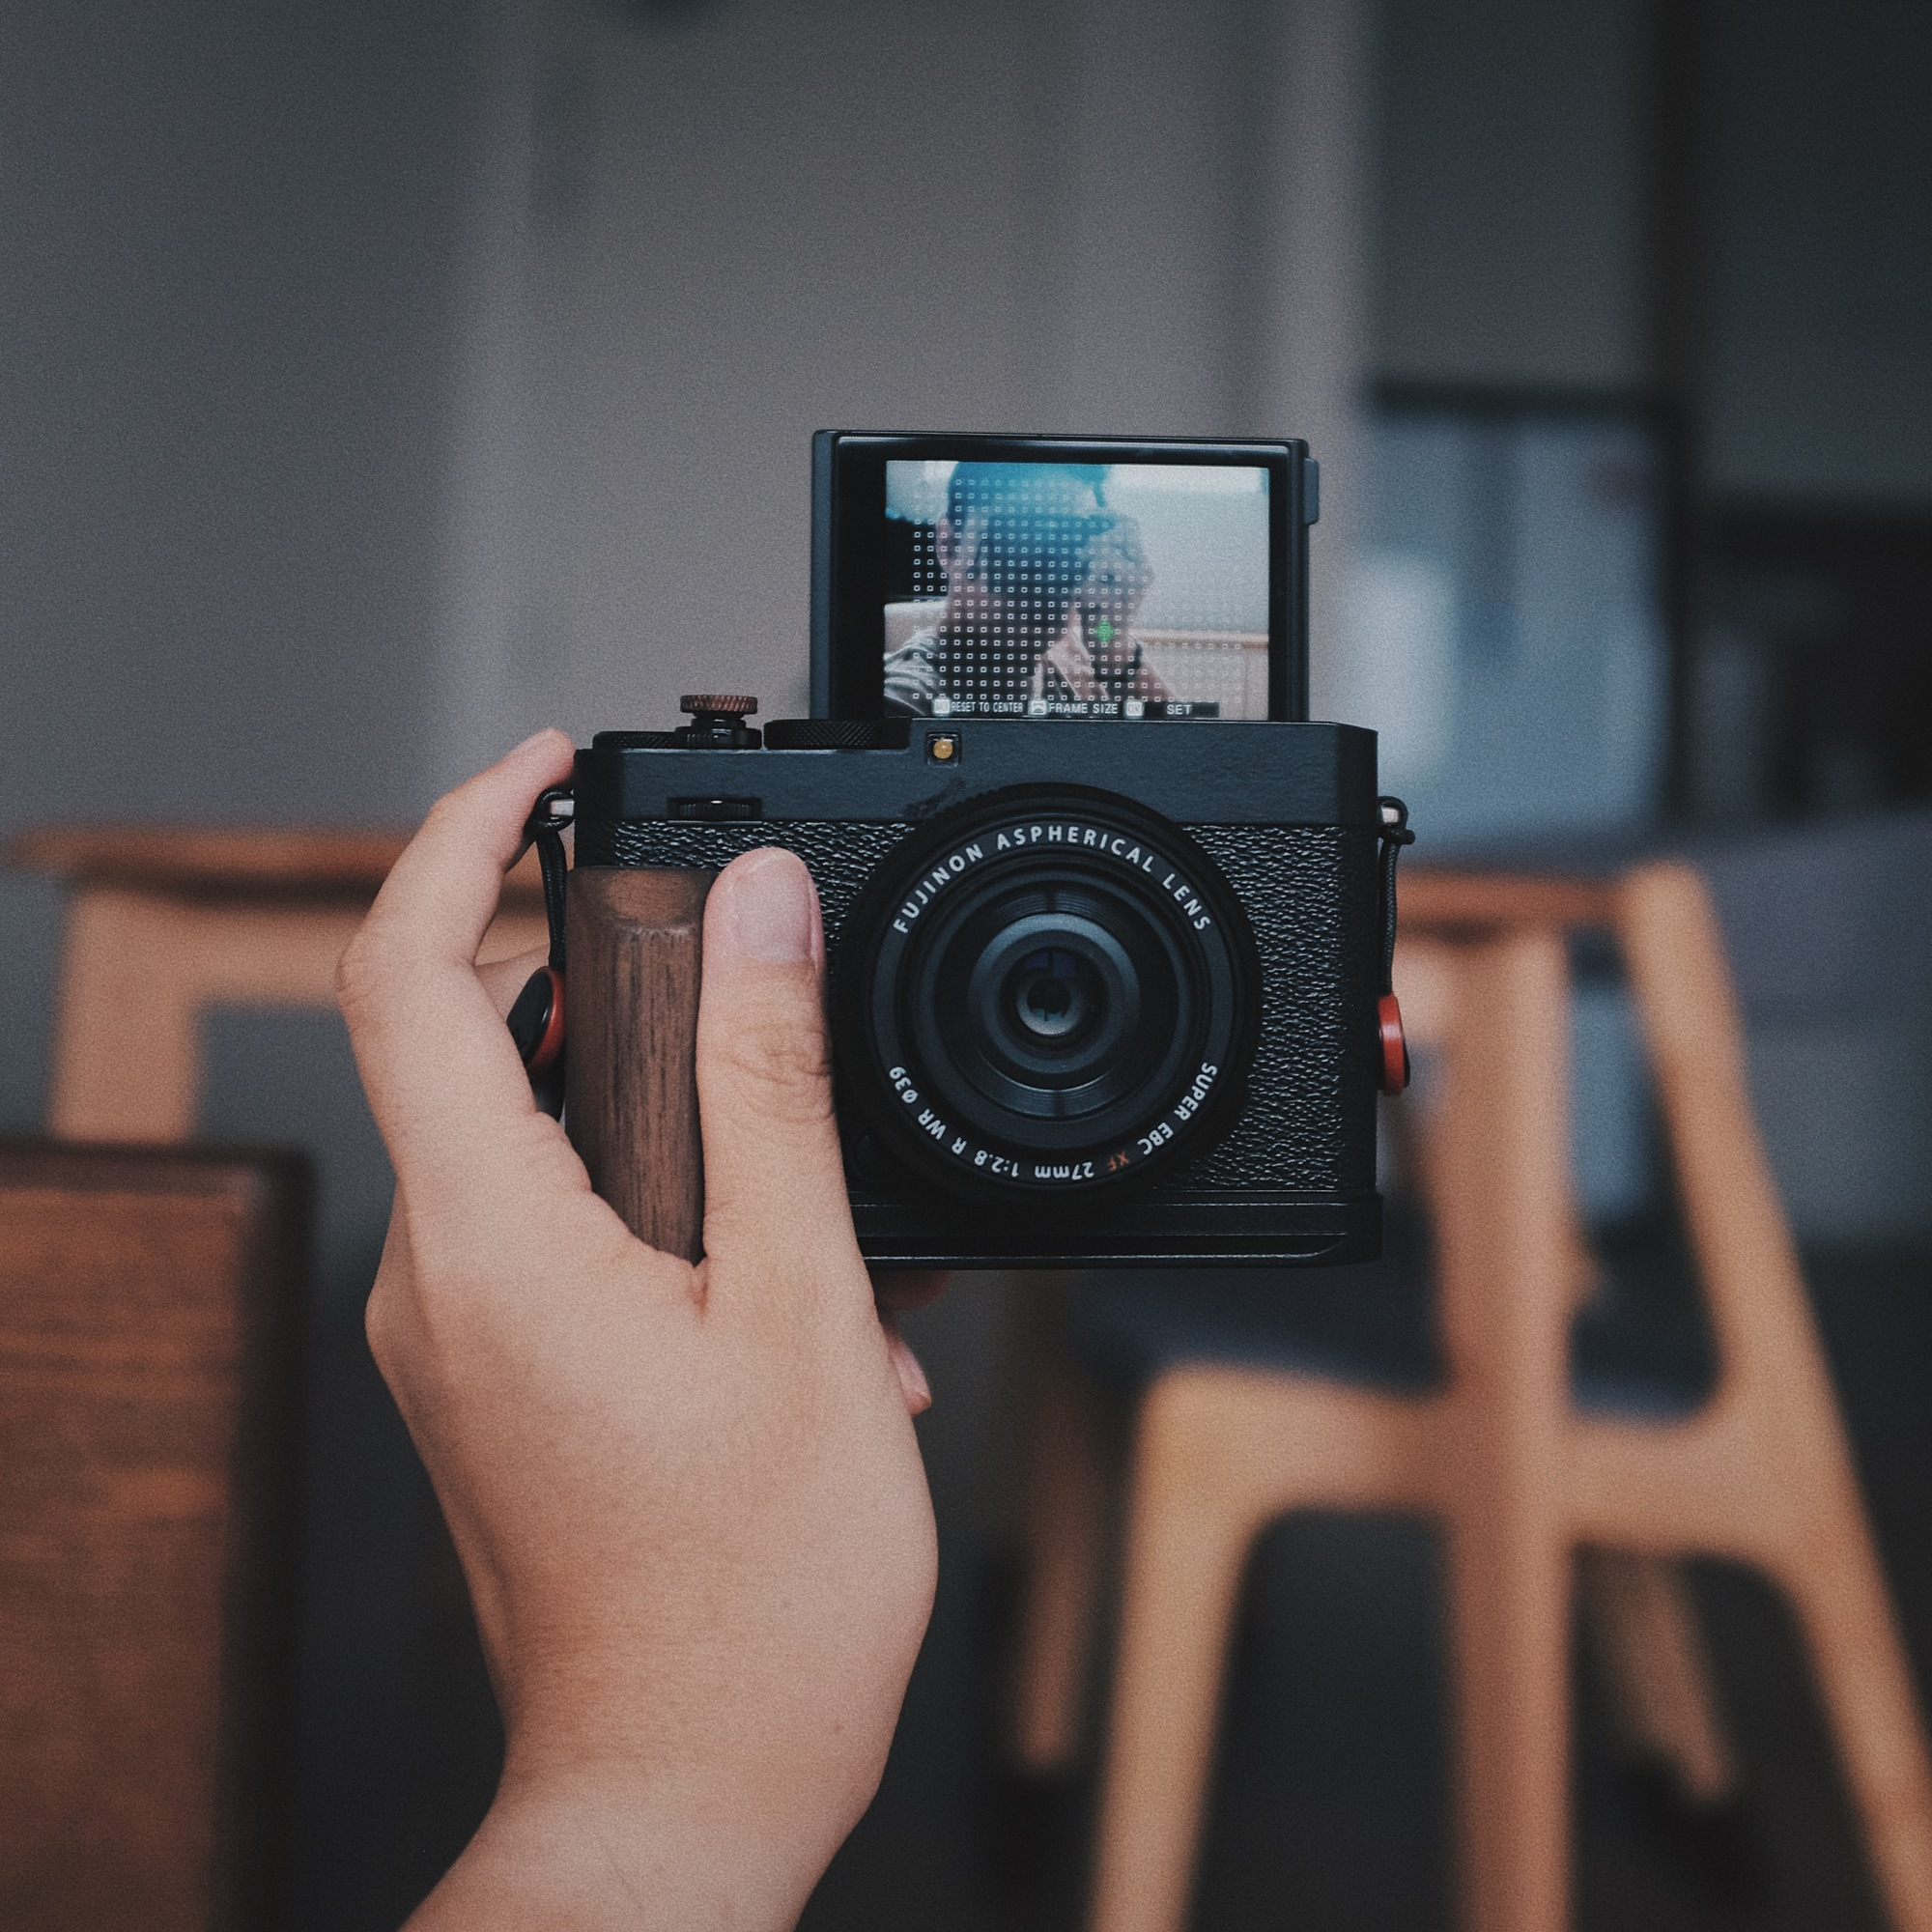
\includegraphics[width=\linewidth]{\envfinaldir/coverpic-prod.jpg}\par
            % \vskip 30pt
            \vfill

            \normalsize\rmfamily\scshape
            \copyright{} The Web Digest Project \hfill\large \envdatestr
        \end{center}
    \end{titlepage}
    % \restoregeometry
}
\newcommand{\simplehref}[1]{%
    \textcolor{blue!80!green}{\href{#1}{#1}}%
}
\renewcommand{\contentsname}{\center\Huge\sffamily\bfseries Contents\par\vskip 20pt}
\newcounter{ipartcounter}
\setcounter{ipartcounter}{0}
\newcommand{\ipart}[1]{
    % \vskip 20pt
    \clearpage
    \stepcounter{ipartcounter}
    \phantomsection
    \addcontentsline{toc}{chapter}{#1}
    % \begin{center}
    %     \Huge
    %     \sffamily\bfseries
    %     #1
    % \end{center}
    % \vskip 20pt plus 7pt
}
\newcounter{ichaptercounter}
\setcounter{ichaptercounter}{0}
\newcommand{\ichapter}[1]{
    % \vskip 20pt
    \clearpage
    \stepcounter{ichaptercounter}
    \phantomsection
    \addcontentsline{toc}{section}{\numberline{\arabic{ichaptercounter}}#1}
    \begin{center}
        \Huge
        \sffamily\bfseries
        #1
    \end{center}
    \vskip 20pt plus 7pt
}
\newcommand{\entrytitlefont}[1]{\subsection*{\raggedright\Large\sffamily\bfseries#1}}
\newcommand{\entryitemGeneric}[2]{
    % argv: title, url
    \parbox{\linewidth}{
        \entrytitlefont{#1}\par\vskip 5pt
        \footnotesize\ttfamily\mdseries
        \simplehref{#2}
    }\vskip 11pt plus 11pt minus 1pt
}
\newcommand{\entryitemGithub}[3]{
    % argv: title, url, desc
    \parbox{\linewidth}{
        \entrytitlefont{#1}\par\vskip 5pt
        \footnotesize\ttfamily\mdseries
        \simplehref{#2}\par\vskip 5pt
        \small\rmfamily\mdseries#3
    }\vskip 11pt plus 11pt minus 1pt
}
\newcommand{\entryitemAp}[3]{
    % argv: title, url, desc
    \parbox{\linewidth}{
        \entrytitlefont{#1}\par\vskip 5pt
        \footnotesize\ttfamily\mdseries
        \simplehref{#2}\par\vskip 5pt
        \small\rmfamily\mdseries#3
    }\vskip 11pt plus 11pt minus 1pt
}
\newcommand{\entryitemHackernews}[3]{
    % argv: title, hnurl, rawurl
    % \parbox{\linewidth}{
    %     \entrytitlefont{#1}\par\vskip 5pt
    %     \footnotesize\ttfamily\mdseries
    %     \simplehref{#3}\par
    %     \textcolor{black!50}{\href{#2}{#2}}
    % }\vskip 11pt plus 11pt minus 1pt
    \begin{minipage}{\linewidth}
            \entrytitlefont{#1}\par\vskip 5pt
            \footnotesize\ttfamily\mdseries
            \simplehref{#3}\par
            \textcolor{black!50}{\href{#2}{#2}}
    \end{minipage}\par\vskip 11pt plus 11pt minus 1pt
}







\begin{document}

\makeheader

\tableofcontents\clearpage




\ipart{Developers}
\ichapter{Hacker News}
\entryitemTwoLinks{Massive Attack turns concert into facial recognition surveillance experiment}{https://news.ycombinator.com/item?id=45255400}{https://www.gadgetreview.com/massive-attack-turns-concert-into-facial-recognition-surveillance-experiment}

\entryitemTwoLinks{William Gibson Reads Neuromancer (2004)}{https://news.ycombinator.com/item?id=45255137}{http://bearcave.com/bookrev/neuromancer/neuromancer\_audio.html}

\entryitemTwoLinks{Addendum to GPT-5 system card: GPT-5-Codex}{https://news.ycombinator.com/item?id=45253458}{https://openai.com/index/gpt-5-system-card-addendum-gpt-5-codex/}

\entryitemTwoLinks{Hosting a website on a disposable vape}{https://news.ycombinator.com/item?id=45252817}{https://bogdanthegeek.github.io/blog/projects/vapeserver/}

\entryitemTwoLinks{React is winning by default and slowing innovation}{https://news.ycombinator.com/item?id=45252715}{https://www.lorenstew.art/blog/react-won-by-default/}

\entryitemTwoLinks{macOS Tahoe}{https://news.ycombinator.com/item?id=45252378}{https://www.apple.com/os/macos/}

\entryitemTwoLinks{GPT-5-Codex}{https://news.ycombinator.com/item?id=45252301}{https://openai.com/index/introducing-upgrades-to-codex/}

\entryitemTwoLinks{Wanted to spy on my dog, ended up spying on TP-Link}{https://news.ycombinator.com/item?id=45251690}{https://kennedn.com/blog/posts/tapo/}

\entryitemTwoLinks{Microsoft to force install the Microsoft 365 Copilot app in October}{https://news.ycombinator.com/item?id=45251593}{https://www.bleepingcomputer.com/news/microsoft/microsoft-to-force-install-the-microsoft-365-copilot-app-in-october/}

\entryitemTwoLinks{Asciinema CLI 3.0 rewritten in Rust, adds live streaming, upgrades file format}{https://news.ycombinator.com/item?id=45251375}{https://blog.asciinema.org/post/three-point-o/}

\entryitemTwoLinks{US lawmakers introduce bill to strip citizens of passports over Israel criticism}{https://news.ycombinator.com/item?id=45251124}{https://thecradle.co/articles-id/33135}

\entryitemTwoLinks{Launch HN: Trigger.dev (YC W23) – Open-source platform to build reliable AI apps}{https://news.ycombinator.com/item?id=45250720}{https://news.ycombinator.com/item?id=45250720}

\entryitemTwoLinks{Paid \$2400 to Cloudflare, support refuses to help}{https://news.ycombinator.com/item?id=45250553}{https://news.ycombinator.com/item?id=45250553}

\entryitemTwoLinks{Meta bypassed Apple privacy protections, claims former employee}{https://news.ycombinator.com/item?id=45250500}{https://9to5mac.com/2025/08/21/meta-allegedly-bypassed-apple-privacy-measure-and-fired-employee-who-flagged-it/}

\entryitemTwoLinks{Apple has a private CSS property to add Liquid Glass effects to web content}{https://news.ycombinator.com/item?id=45250370}{https://alastair.is/apple-has-a-private-css-property-to-add-liquid-glass-effects-to-web-content/}

\entryitemTwoLinks{How to self-host a web font from Google Fonts}{https://news.ycombinator.com/item?id=45250202}{https://blog.velocifyer.com/Posts/3,0,0,2025-8-13,+how+to+self+host+a+font+from+google+fonts.html}

\entryitemTwoLinks{PayPal to support Ethereum and Bitcoin}{https://news.ycombinator.com/item?id=45249915}{https://newsroom.paypal-corp.com/2025-09-15-PayPal-Ushers-in-a-New-Era-of-Peer-to-Peer-Payments,-Reimagining-How-Money-Moves-to-Anyone,-Anywhere}

\entryitemTwoLinks{CubeSats are fascinating learning tools for space}{https://news.ycombinator.com/item?id=45249878}{https://www.jeffgeerling.com/blog/2025/cubesats-are-fascinating-learning-tools-space}

\entryitemTwoLinks{Hosting a website on a disposable vape}{https://news.ycombinator.com/item?id=45249287}{https://bogdanthegeek.github.io/blog/projects/vapeserver/}

\entryitemTwoLinks{How big a solar battery do I need to store all my home's electricity?}{https://news.ycombinator.com/item?id=45248899}{https://shkspr.mobi/blog/2025/09/how-big-a-solar-battery-do-i-need-to-store-all-my-homes-electricity/}\ichapter{Phoronix}
\entryitemGeneric{\hskip 0pt{}Godot 4.5 Open-Source Game Engine Released With A Multitude Of Improvements}{https://www.phoronix.com/news/Godot-4.5-Released}

\entryitemGeneric{\hskip 0pt{}AMD ABMC Expected To Go Upstream For Linux 6.18}{https://www.phoronix.com/news/AMD-ABMC-TIP-Queued}

\entryitemGeneric{\hskip 0pt{}AOMedia To Release AV2 Video Codec At Year's End}{https://www.phoronix.com/news/AOMedia-AV2-Coming-Soon}

\entryitemGeneric{\hskip 0pt{}AMD Officially Confirms The End Of The AMDVLK Driver}{https://www.phoronix.com/news/AMDVLK-Discontinued}

\entryitemGeneric{\hskip 0pt{}libxml2 Maintainer Stepping Down - "More Or Less Unmaintained For Now"}{https://www.phoronix.com/news/Libxml2-No-Maintainer}

\entryitemGeneric{\hskip 0pt{}The Performance Cost To Ubuntu WSL2 On Windows 11 25H2}{https://www.phoronix.com/review/windows-11-wsl2-2025}

\entryitemGeneric{\hskip 0pt{}Canonical Announces Plans To Support NVIDIA CUDA, Easy Installation On Ubuntu}{https://www.phoronix.com/news/Ubuntu-Better-CUDA}

\entryitemGeneric{\hskip 0pt{}Casilda 1.0 Released As Wayland Compositor Widget For GTK4}{https://www.phoronix.com/news/Casilda-1.0-Wayland-GTK4}

\entryitemGeneric{\hskip 0pt{}Jonathan Riddell Leaving KDE Development After 25 Years}{https://www.phoronix.com/news/Riddell-Leaves-KDE}


\ipart{Developers~~~~(zh-Hans)}
\ichapter{Solidot}
\entryitemGeneric{\hskip 0pt{}韩国扫地机器人试图通过差异化与中国公司竞争}{https://www.solidot.org/story?sid=82315}

\entryitemGeneric{\hskip 0pt{}全球人口正以更快的速度收缩}{https://www.solidot.org/story?sid=82314}

\entryitemGeneric{\hskip 0pt{}日本老年人口比例占到 29.4\%}{https://www.solidot.org/story?sid=82313}

\entryitemGeneric{\hskip 0pt{}CRISPR 基因编辑的马引发争议}{https://www.solidot.org/story?sid=82312}

\entryitemGeneric{\hskip 0pt{}日本百岁人口数量接近 10 万}{https://www.solidot.org/story?sid=82311}

\entryitemGeneric{\hskip 0pt{}NewsGuard 的调查显示 AI 生成虚假信息的比例一年内翻了一倍}{https://www.solidot.org/story?sid=82310}

\entryitemGeneric{\hskip 0pt{}AMD 的 RDNA4 GPU 架构}{https://www.solidot.org/story?sid=82309}

\entryitemGeneric{\hskip 0pt{}2025 年度拉斯克医学奖揭晓}{https://www.solidot.org/story?sid=82308}

\entryitemGeneric{\hskip 0pt{}阿联酋发布能与 DeepSeek 竞争的开源模型}{https://www.solidot.org/story?sid=82307}

\entryitemGeneric{\hskip 0pt{}照片显示缅甸电诈园区的面积仍然在扩大}{https://www.solidot.org/story?sid=82306}

\entryitemGeneric{\hskip 0pt{}美国啤酒 95\% 含有 PFAS}{https://www.solidot.org/story?sid=82305}

\entryitemGeneric{\hskip 0pt{}社交媒体的末日}{https://www.solidot.org/story?sid=82304}

\entryitemGeneric{\hskip 0pt{}互联网档案馆保存的网页数即将突破 1 万亿}{https://www.solidot.org/story?sid=82303}

\entryitemGeneric{\hskip 0pt{}尼泊尔 Z 世代抗议中的技术力量}{https://www.solidot.org/story?sid=82302}

\entryitemGeneric{\hskip 0pt{}Proton Mail 应网络安全机构要求关闭了记者账户}{https://www.solidot.org/story?sid=82301}

\entryitemGeneric{\hskip 0pt{}中国电动汽车技术如何重塑全球汽车设计}{https://www.solidot.org/story?sid=82300}\ichapter{V2EX}
\entryitemGeneric{\hskip 0pt{}[iOS] iOS26 那个预览 app 要接受打开么?}{https://www.v2ex.com/t/1159479}

\entryitemGeneric{\hskip 0pt{}[Apple] iOS26 有两套键盘图标,太割裂了吧}{https://www.v2ex.com/t/1159478}

\entryitemGeneric{\hskip 0pt{}[MacBook Pro] 16 寸 MacBook Pro,要等 M5 吗}{https://www.v2ex.com/t/1159477}

\entryitemGeneric{\hskip 0pt{}[Apple] 等一个会开启 macOS26 和 iOS26 国际版地图的人}{https://www.v2ex.com/t/1159476}

\entryitemGeneric{\hskip 0pt{}[Apple] iOS 26 后绕过 Wi-Fi Calling 地区限制的方法可能不再有效}{https://www.v2ex.com/t/1159475}

\entryitemGeneric{\hskip 0pt{}[Bing] 比百度还哈人}{https://www.v2ex.com/t/1159474}

\entryitemGeneric{\hskip 0pt{}[iOS] iOS26 通知栏下滑行程好长}{https://www.v2ex.com/t/1159473}

\entryitemGeneric{\hskip 0pt{}[Apple] macos26 屏幕保护程序存在 bug}{https://www.v2ex.com/t/1159472}

\entryitemGeneric{\hskip 0pt{}[问与答] 高中社团活动日想在摊位的大屏展示一些有趣的吸引学生的程序,大家有推荐吗?}{https://www.v2ex.com/t/1159471}

\entryitemGeneric{\hskip 0pt{}[Apple] iOS 26 已更新,开个反馈帖}{https://www.v2ex.com/t/1159470}

\entryitemGeneric{\hskip 0pt{}[TypeScript] TypeScript5.9,仿佛走出草原来到了现代社会}{https://www.v2ex.com/t/1159469}

\entryitemGeneric{\hskip 0pt{}[Apple] 等半天没见 macos26,却出来个 15.67}{https://www.v2ex.com/t/1159468}

\entryitemGeneric{\hskip 0pt{}[分享创造] 有没有人玩过皇室战争卡牌猜词游戏 Clash Royale card guessing game}{https://www.v2ex.com/t/1159467}

\entryitemGeneric{\hskip 0pt{}[AirPods] 今天又把 AirPods Pro2 返厂了}{https://www.v2ex.com/t/1159466}

\entryitemGeneric{\hskip 0pt{}[小米] 建议小米将 xiaomi 改名为 MiPhone,将澎湃 OS 改名为 MiOS}{https://www.v2ex.com/t/1159463}

\entryitemGeneric{\hskip 0pt{}[随想] 悲哀的发现人想过的好就必须卷。}{https://www.v2ex.com/t/1159461}

\entryitemGeneric{\hskip 0pt{}[生活] [相亲]还没见过面,就开始想着带人家出去玩?}{https://www.v2ex.com/t/1159460}

\entryitemGeneric{\hskip 0pt{}[Apple] 突然发现 eSIM 全面普及后会更容易限制国内用户购买非国行终端}{https://www.v2ex.com/t/1159459}

\entryitemGeneric{\hskip 0pt{}[生活] 邀请各位赐教人生之路的选择与讨论—— [稳定] 或 [高薪]}{https://www.v2ex.com/t/1159458}

\entryitemGeneric{\hskip 0pt{}[程序员] 长时间不关电脑网速下降}{https://www.v2ex.com/t/1159454}

\entryitemGeneric{\hskip 0pt{}[问与答] 有兄弟买了 amd 的 aimax 395 吗?}{https://www.v2ex.com/t/1159453}

\entryitemGeneric{\hskip 0pt{}[YouTube] 求救,频道会员的支付遇到问题了}{https://www.v2ex.com/t/1159451}

\entryitemGeneric{\hskip 0pt{}[生活] 停路边划线车位, 车被人暗算了}{https://www.v2ex.com/t/1159450}

\entryitemGeneric{\hskip 0pt{}[酷工作] [北京] [Golang] 招聘 高级后端开发 30K ~ 60K}{https://www.v2ex.com/t/1159449}

\entryitemGeneric{\hskip 0pt{}[问与答] 国内的中央厨房到底长什么样子?}{https://www.v2ex.com/t/1159448}

\entryitemGeneric{\hskip 0pt{}[Cursor] cursor 的 claude-4-sonnet-1m 模型好变态,消耗速度飞快。两百多请求不到两小时给干完}{https://www.v2ex.com/t/1159447}

\entryitemGeneric{\hskip 0pt{}[宽带症候群] 成都移动改了路由器拨号网变卡}{https://www.v2ex.com/t/1159446}

\entryitemGeneric{\hskip 0pt{}[iCloud] 云上贵州 icloud.com.cn 每次登入你们有没有邮箱提示记录?}{https://www.v2ex.com/t/1159445}

\entryitemGeneric{\hskip 0pt{}[酷工作] 小红书客户端基建招人,坑位多多,欢迎来投}{https://www.v2ex.com/t/1159444}

\entryitemGeneric{\hskip 0pt{}[日本] 国庆赴日游,有什么 tip 提供吗}{https://www.v2ex.com/t/1159443}

\entryitemGeneric{\hskip 0pt{}[加密货币] Boost 第二期来了!}{https://www.v2ex.com/t/1159442}

\entryitemGeneric{\hskip 0pt{}[问与答] 想练练左手拿鼠标,有没有办法快速设置适合右手操作的复制粘贴快捷键?}{https://www.v2ex.com/t/1159440}

\entryitemGeneric{\hskip 0pt{}[问与答] 这是新型骗局吗}{https://www.v2ex.com/t/1159439}

\entryitemGeneric{\hskip 0pt{}[推广] 最近发现一个叫 Dahej Calculator 嫁妆计算器的,主要访问国家是印度}{https://www.v2ex.com/t/1159438}

\entryitemGeneric{\hskip 0pt{}[投资] 卖了特斯拉,特斯拉一直涨,心态崩了}{https://www.v2ex.com/t/1159437}

\entryitemGeneric{\hskip 0pt{}[分享创造] 使用 Claude Cli 构建的一个试验性站点,感叹下 Claude 的高效}{https://www.v2ex.com/t/1159436}

\entryitemGeneric{\hskip 0pt{}[职场话题] 嵌入式软件开发, 47 岁牛马,接着卷。。}{https://www.v2ex.com/t/1159434}

\entryitemGeneric{\hskip 0pt{}[程序员] AI 赛事通 - 2025 年 8 月 AI 竞赛汇总合集}{https://www.v2ex.com/t/1159433}

\entryitemGeneric{\hskip 0pt{}[DotA] 作为阿森纳(英超三连亚)和 CNDOTA(亚了不知道多少年了)的支持者,我可能有着世界上最好的心态。}{https://www.v2ex.com/t/1159431}

\entryitemGeneric{\hskip 0pt{}[小米] 有懂充电宝的兄弟吗?}{https://www.v2ex.com/t/1159428}

\entryitemGeneric{\hskip 0pt{}[Apple] 分享自己与 Apple 客服沟通的小记,非常感谢苹果的技术支持}{https://www.v2ex.com/t/1159427}

\entryitemGeneric{\hskip 0pt{}[English] 有没有学英语的播客推荐}{https://www.v2ex.com/t/1159426}

\entryitemGeneric{\hskip 0pt{}[CDN] 有没有分销 Cloudflare 企业版的}{https://www.v2ex.com/t/1159425}

\entryitemGeneric{\hskip 0pt{}[Python] Celery 不支持类方法吗?静态方法呢}{https://www.v2ex.com/t/1159424}

\entryitemGeneric{\hskip 0pt{}[分享发现] v2er 更新了,好耶😆}{https://www.v2ex.com/t/1159423}

\entryitemGeneric{\hskip 0pt{}[问与答] 小米真就这么没自信吗?连名字也要蹭??}{https://www.v2ex.com/t/1159422}

\entryitemGeneric{\hskip 0pt{}[Solana] 增持 10💎后 177💎大佬 bZpa 砸盘}{https://www.v2ex.com/t/1159420}

\entryitemGeneric{\hskip 0pt{}[Solana] 不懂就问, Phantom 钱包有 USDT,怎么付款}{https://www.v2ex.com/t/1159419}

\entryitemGeneric{\hskip 0pt{}[分享创造] 做了一个文本转多人有声剧的 AI 工具}{https://www.v2ex.com/t/1159418}

\entryitemGeneric{\hskip 0pt{}[上海] 下班前往窗外一望,好家伙 nv 和 amd 作伴了}{https://www.v2ex.com/t/1159417}


\ipart{Generic News}







\clearpage
\leavevmode\vfill
\footnotesize

Copyright \copyright{} 2023-2025 Neruthes and other contributors.

This document is published with CC BY-NC-ND 4.0 license.

The entries listed in this newsletter may be copyrighted by their respective creators.

This newsletter is generated by the Web Digest project.

The newsletters are also delivered via Telegram channel \CJKunderline{\href{https://t.me/webdigestchannel}{https://t.me/webdigestchannel}}.\\
RSS feed is available at \CJKunderline{\href{https://webdigest.pages.dev/rss.xml}{https://webdigest.pages.dev/rss.xml}}.

This newsletter is available in PDF at
\CJKunderline{\href{https://webdigest.pages.dev/}{https://webdigest.pages.dev/}}.

The source code being used to generate this newsletter is available at\\
\CJKunderline{\href{https://github.com/neruthes/webdigest}{https://github.com/neruthes/webdigest}}.

This newsletter is also available in
\CJKunderline{\href{http://webdigest.pages.dev/readhtml/\envyear/WebDigest-20250916.html}{HTML}} and
\CJKunderline{\href{https://github.com/neruthes/webdigest/blob/master/markdown/\envyear/WebDigest-20250916.md}{Markdown}}.


\coverpic{https://unsplash.com/photos/palm-trees-frame-a-dramatic-mountain-valley-landscape-dw21nYHrCx4}{Kiril Krsteski}


\end{document}
